\documentclass[lettersize,journal]{IEEEtran}
\usepackage{amsmath,amsfonts}
\usepackage{algorithmic}
\usepackage{algorithm}
\usepackage{array}
\usepackage[caption=false,font=normalsize,labelfont=sf,textfont=sf]{subfig}
\usepackage{textcomp}
\usepackage{stfloats}
\usepackage{url}
\usepackage{verbatim}
\usepackage{graphicx}
\usepackage{cite}
\usepackage{longtable} % for tables
\usepackage{booktabs} % for tables

\hyphenation{op-tical net-works}
\setlength{\parindent}{0pt}

\begin{document}

\title{Neural Networks-Deep Learning \\ 2nd Assignment}
\author{Papadakis Konstantinos Fotios}
% The paper headers
\markboth{Neural Networks-Deep Learning, 2nd Assignment, 2024}
\maketitle

\begin{abstract}
This is the second Assignment of the course "Neural Networks-Deep Learning". It revolves around
creating a Support Vector Machine and and training it on the CIFAR-10 dataset to successfully 
classify the images into one of the 10 classes. The algorithm used is analyzed extensively and
results both in the testing and training phase are presented. SVM is challenged by other similar
algorithms that are also trained on the CiFAR-10 dataset and try to solve the same classification 
problem. These rival algorithms include 1 and 3 Nearest Neighbor, Nearest Centroid and MLP with
one hidden layer using Hinge loss.
\end{abstract}

\section{Introduction}
\IEEEPARstart{T}{he} second assignment is going to utilize results from the first assignment and
thus the dataset has to be the same: "CIFAR-10".
\begin{itemize}
  \item \url{https://www.cs.toronto.edu/~kriz/cifar.html}
\end{itemize}

It consists of 60000 32x32 color images which belong to one of the 10 available classes. There are
6000 images per class, 5000 training images and 1000 test images. The data is available in 6 
batches of 10000 images each.
\begin{itemize}
  \item five training batches (50,000 or 5000 images from each class)
  \item one test batch (10,000 or 1000 images from each class)
\end{itemize}
Since the training batches' images are chosen randomly, each batch individually may contain more 
images from one class than another but, cumulatively, the number of images from each class is 
equal. Here is an example of the dataset's structure:

\begin{figure}[H]
  \centering
  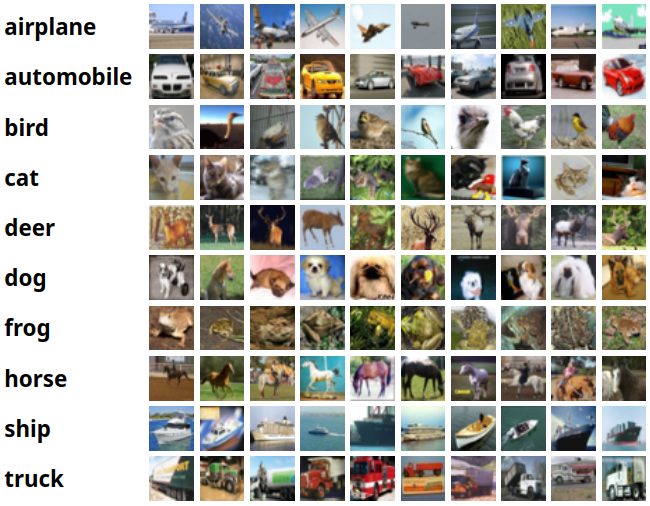
\includegraphics[width=2.5in]{media/cifar10_example.png}
  \caption{The CIFAR-10 dataset.}
  \label{CIFAR example}
\end{figure} 

\section{Support Vector Machine}
Support Vector Machines are supervised maximum margin models that are used for problems 
such as:
\begin{itemize}
    \item Classification
    \item Regression
    \item Distribution Estimation
\end{itemize}
They are considered supervised because they need a pre-labeled training set to develop 
the hyperplanes that separate the classes. The terminology maximum margin refers to the
fact that the SVM tries to solve a convex optimization problem which maximizes the 
distance between the hyperplane and the closest data points from each class. This 
distance is called "margin".

\begin{figure}[H]
    \centering
    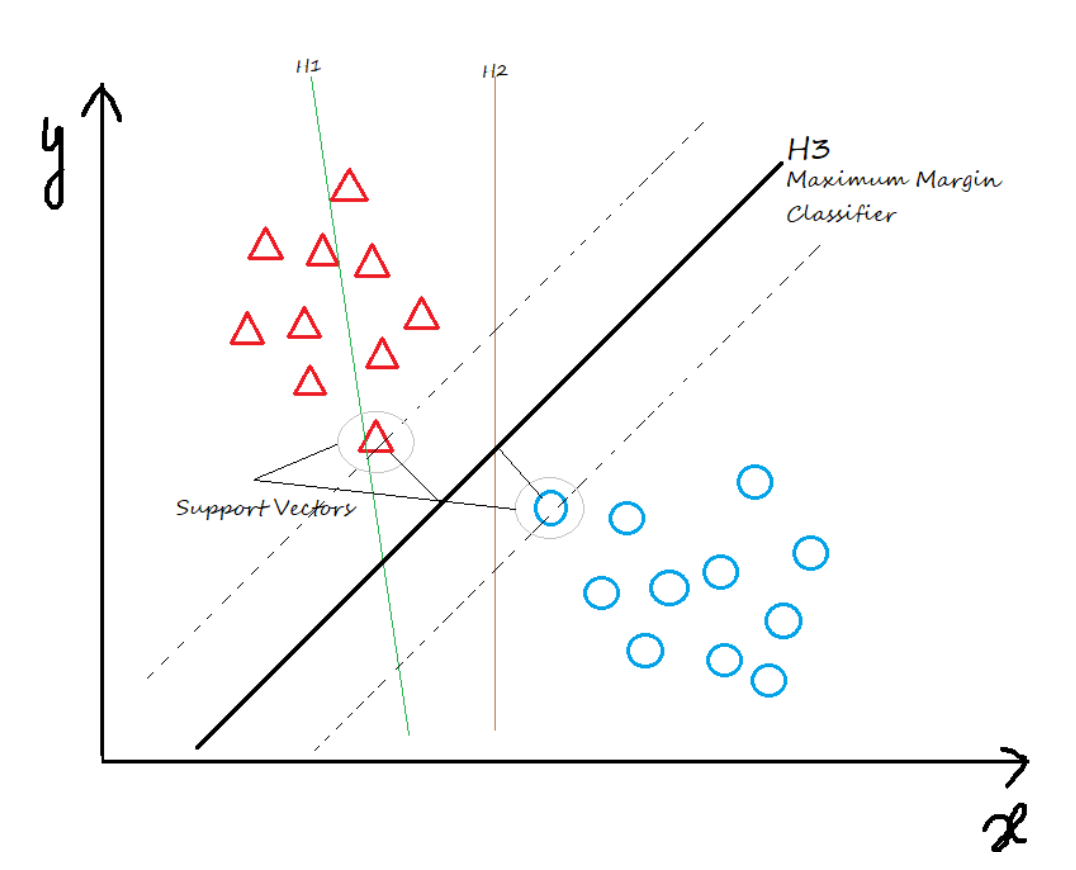
\includegraphics[width=0.5\textwidth]{media/svm_example.png}
    \caption{SVM Maximum Margin Classifier}
\end{figure}


\section{Multi-Layer Perceptron}
Another model with which we have worked on the first assignment is MLP also known as 
Multi-Layer Perceptron. One aspect in which we are going to divert from the first 
assignment's implementation, is the loss function. Here we will be using the Hinge loss 
function which is going to allow us to directly compare the MLP with the SVM.
    
\subsection{}
\subsection{Hinge Loss}

\section{Nearest Neighbor and Nearest Centroid}
First nearest neighbor, third nearest neighbor and nearest centroid are three basic
classification algorithms we will be taking from the first assignment to compare our
SVM with. These as we have explained previously are algorithms that classify by:
\begin{itemize}
    \item Nearest Neighbor: Assigns to the test point the class of the nearest to it 
    centroid calculated from all the points in the training dataset. 
    \item 1 Nearest Centroid: Assigns to the test point the class of the closest to it 
    point from the training dataset.
    \item 3 Nearest Neighbor: Assigns to the test point the average class of the closest
    to it 3 points from the training dataset.
\end{itemize}

\section{Results}
\subsection{Comparison of Algorithms}
\input{sections/comp.tex}

\vfill
\end{document}


